\chapter*{Probabilistic Bayesian Filtering}
\section{Introduction}
In this chapter the theory of probabilistic Bayesian filtering (PBF) is presented. The Kalman filtering equations, which are the closed form solutions to the linear Gaussian discrete-time optimal filtering problem, are also derived.

\section{Probabilistic Filtering Equations and Exact Solutions}
Before going into the practical non-linear filtering algorithms, we first present the classical formulation of the discrete-time optimal filtering as recursive Bayesian inference. Then the classical Kalman filters, extended Kalman filters and statistical linearization based filters are presented in terms of the general theory. 
\newtheorem {thm}{Definition}[section]

\begin{thm}[State space model]. 
Discrete-time state space model or probabilistic non-linear filtering model is a recursively defined probabilistic model of the form

\begin{eqnarray} \label{eqn: State space model}
x_k & \approx & p(x_k | x_{k-1} ) \nonumber \\
y_k &  \approx & p(y_k | x_k ) 
\end{eqnarray}

where:

\begin{itemize}
\item $x_k \in \Re_{n}$ is the state of the system on the time step $k$.
\item $y_k \in \Re_{n}$ is the measurement on the time step $k$.
\item $p(x_k | x_{k-1})$ is the dynamic model, which models the stochastic dynamics of the system. The dynamic model can be a probability density, a counting measure or combination of them depending on if the state $x_k$ is continuous, discrete or hybrid.
\item $p(y_k | x_k )$ is the measurement model, which models the distribution of the
measurements given the state.
\end{itemize}

\end{thm}

The model is assumed to be Markovian, which means that it has the following two properties:
\newtheorem{thm1}{Property}[section]

\begin{thm1} [Markov property of states]
States $\{x_k : k = 1, 2, . . .\}$ form a Markov sequence (or Markov chain if the state
is discrete). This Markov property means that $x_k$ (and actually the whole future
$(x_{k+1} , x_{k+2} , . . .)$ given $x_{k-1}$ is independent from anything that has happened in the past:

\begin{eqnarray} \label{eqn: Indipendence State1}
p(x_k | x_{1:k−1} , y_{1:k−1} ) = p(x_k | x_{k-1} ).
\end{eqnarray}

Also the past is independent of the future given the present:
\begin{eqnarray} \label{eqn: Indipendence State2}
p(x_{k-1} | x_{k:T} , y_{k:T} ) = p(x_{k-1} | x_k ).
\end{eqnarray}
\end{thm1} 

\newtheorem{thm2}{Property}[section]

\begin{thm2} [Conditional independence of mesaurements]
The measurement $y_k$ given the state $x_k$ is conditionally independent from the mea-
surement and state histories:
 \begin{eqnarray} \label{eqn: Indipendence Measurement}
 p(y_{k} | x_{1:k} , y_{1:k-1} ) = p(y_k | x_k ).
 \end{eqnarray}
\end{thm2}

The filtering model can be equivalently expressed as an Hidden Markov chain or a directed  graphical model whose representation is depicted in figure \ref{fig:GM}
\begin{figure}[!htb]\label{fig:GM}
\begin{center}
 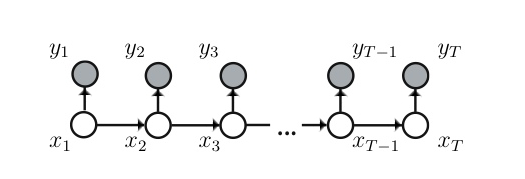
\includegraphics[width=10cm]{./ImaginiLatex/gm_directed.eps} 
\end{center}
\caption{The directed graph of the Filtering Model. The link  $x_k$ and $x_{k-1}$ express the markov property while the link between $y_k$ and $x_k$ express the conditional indipendence property of measurements}

\end{figure}

Following the factorization theorem for the directed graphical models:
\begin{eqnarray} \label{eqn: Full Joint Distribution}
p(x_0 , . . . , x_T,y_1 , . . . , y_T ) = p(x_0 ) \prod_{k=1}^{T} p(x_k | x_{k-1} ) = \nonumber \\
\prod_{k=1}^{T} p(y_k | x_{k} ) 
\end{eqnarray}

Marginalizing out $Y=\{y_1 , . . . , y_T\}$ from the joint distribution we obtain
the joint prior distribution of the states $X={x_0 , . . . , x_T}$ :
\begin{eqnarray} \label{eqn: joint states distribution}
p(x_0 , . . . , x_T ) = \int p(y_1 , . . ,y_T , x_1 , . ., x_T) d(y_1 , . ., y_T) =  \nonumber \\
p(x_0 ) \prod_{k=1}^{T} p(x_k | x_{k - 1} ) 
\end{eqnarray}

Applying the bayes rule to \ref{eqn: Full Joint Distribution} and \ref{eqn: joint states distribution} we can compute the joint likelihood of measurements $Y=\{y_1 , . . . , y_T\}$:
\begin{eqnarray} \label{eqn: joint measurements likelyhood}
p(y_1 , . . . , y_T | x_0 , . . . , x_T ) = \nonumber \\
\frac{p(y_1 , . . ,y_T,x_1 , . ., x_T)}{ p(x_0,x_1 , . ., x_T)} = \nonumber \\
\prod_{k=1}^{T} p(y_k | x_k) 
\end{eqnarray}

In principle, for given $T$ we could simply compute the posterior distribution of the
states by the Bayes rule:

\begin{eqnarray}  \label{eqn: Bayes rule2}
p(x_0,x_1 , x_2 , . . x_T | y_1 , y_2 , . . ,y_T)= 
\frac{ p(y_1 , . . ,y_T | x_1 , . ., x_T )p(x_1 , . . ,x_T) } {p(y_1,..,y_T)} \nonumber \\
\approx p(y_1 , . . ,y_T | x_1 , . ., x_T  ) p(x_1 , . . ,x_T)
\end{eqnarray}

However, this kind of explicit usage of the full Bayes’ rule is not feasible in real
time applications, because the amount of computations per time step increases
when new observations arrive. Thus, this way we could only work with small data
sets, because if the amount of data is not bounded (as in real time sensoring appli-
cations), then at some point of time the computations would become intractable.
To cope with real time data we need to have an algorithm which does constant
amount of computations per time step.
As discussed in Section 1.2.3, filtering distributions, prediction distributions
and smoothing distributions can be computed recursively such that only constant
amount of computations is done on each time step. For this reason we shall not con-
sider the full posterior computation at all, but concentrate to the above-mentioned
distributions instead.

\section{Optimal Filtering Equations}
The purpose of optimal filtering is to compute the marginal posterior distribution
of the state $x_k$ on the time step $k$ given the history of the measurements up to the
time step $k$
\begin{eqnarray} \label{eqn: Optimal Filtering Equations}
p(x_k | y_{1:k} ). 
\end{eqnarray} 

The fundamental equations of the Bayesian filtering theory are given by the fol-
lowing theorem:
\newtheorem{thm3}{Theorem}[section]

\begin{thm3} [Bayesian optimal filtering equations]
The recursive equations for computing the predicted distribution $p(x_k | y_{1:k-1})$ and the filtering distribution $p(x_k | y_{1:k})$ on the time step $k$ are given by the following Bayesian filtering steps:
\begin{enumerate}
\item \textbf{Initialization}. The recursion starts from the prior distribution $p(x_0 )$.
\item \textbf{Prediction}. The predictive distribution of the state $x_k$ on time step $k$ given the dynamic model can be computed by the \textbf{Chapman-Kolmogorov} equation

\begin{eqnarray} \label{eqn: Prediction Step}
p(x_k | y_{1:k-1} ) =p(x_k | x_{k-1} ) p(x_{k-1} | y_{1:k-1} ) dx_{k-1} .
\end{eqnarray}

\item \textbf{Update}. Given the measurement $y_k$ on time step $k$ the posterior distribution of the state $xk$ can be computed by the Bayes’ rule
\begin{eqnarray} \label{eqn: Update Step}
p(x_k | y_{1:k} ) = \frac{1}{Z_k} p(y_k | x_k ) p(x_k | y_{1:k-1} ),
\end{eqnarray}

where the normalization constant $Z_k$ is given as
\begin{eqnarray} \label{eqn: Normalization}
Z_k = p(y_k | x_k ) p(x_k | y_{1:k-1} ) dx_k .
\end{eqnarray}
\end{enumerate}

If some of the components of the state are discrete, the corresponding integrals are
replaced with summations.
\end{thm3}

\textit{Proof.} The joint distribution of $x_k$ and $x_{k-1}$ given $y_{1:k-1}$ can be computed as
\begin{eqnarray} \label{eqn: prof1}
p(x_k , x_{k-1} | y_{1:k-1} ) =   \frac{p(x_k , x_{k-1} , y_{1:k-1})}{p(y_{1:k-1})} = \nonumber \\
\frac{p(x_k | x_{k-1} , y_{1:k-1}) p(x_{k-1} , y_{1:k-1}) }{p(y_{1:k-1})} =
 p(x_k | x_{k-1} , y_{1:k-1}) p(x_{k-1} | y_{1:k-1}) 
\end{eqnarray}

that can be further simplified by the Independence properties of Markov assumption \ref{eqn: Indipendence State1} and \ref{eqn: Indipendence State2} in 
\begin{eqnarray} \label{eqn: prof2}
p(x_k , x_{k-1} | y_{1:k-1} )= p(x_k | x_{k-1} ) p(x_{k-1} | y_{1:k-1} )
\end{eqnarray}


The marginal distribution of $x_k$ given $y_{1:k-1}$ can be obtained marginalizing out the  $x_{k-1}$ from the distribution
\footnote{This arise applying the simple substitution to the joint distribution of 3 events
$A$,$B$ and $C$:
$$
p(A|C)=\int \frac{p(A,B,C)}{p(C)}dB=\frac{1}{p(C)}\int p(A,B,C)dB =\frac{p(A,C)}{p(C)}
$$
} 
 \label{eqn: prof2} giving the Chapman-Kolmogorov equation

\begin{eqnarray} \label{eqn: Chapman-Kolmogorov}
p(x_k | y_{1:k-1} )= \int p(x_k | x_{k-1} ) p(x_{k-1} | y_{1:k-1} ) dx_{k-1}
\end{eqnarray}

If $x_{k-1}$ is discrete, then the above integral is replaced with sum over $x_{k-1}$ .
The normalization factor $Z_k$ in can be expressed as:
\begin{eqnarray} \label{eqn: Normalization1}
Z_k =  p(y_k | y_{1:k-1})= \frac{p(y_k , y_{1:k-1})}{p( y_{1:k-1})} = 
\int \frac{ p( y_k , y_{1:k-1} , x_k) }{ p( y_{1:k-1}) } dx_k =  \\
\int \frac{ p(y_k | x_k , y_{1:k-1}) p(x_k , y_{1:k-1}) }{ p( y_{1:k-1}) } dx_k = 
\int \frac{ p(y_k | x_k) p(x_k , y_{1:k-1}) }{ p( y_{1:k-1}) } dx_k = \\
=\int p(y_k | x_k ) p(x_k | y_{1:k-1} ) dx_k
\end{eqnarray}

The posterior distribution of $x_k$ given $y_k$ and $y_{1:k-1}$ can be computed as:
\begin{eqnarray} \label{eqn: Posterior}
p(x_k | y_{1:k} )=  \frac{ p(x_k , y_k , y_{1:k-1} )}{ p(y_k , y_{1:k-1})} =
 \frac{ p(y_k | x_k , y_{1:k-1}) p(x_k , y_{1:k-1}) }{  p(y_k , y_{1:k-1})} = \\
 \frac{ p(y_k | x_k) p(x_k , y_{1:k-1}) }{ p(y_k , y_{1:k-1}) } =
 \frac{ p(y_k | x_k) p(x_k | y_{1:k-1}) p(y_{1:k-1}) }{ p(y_k , y_{1:k-1}) } = \\
 \frac{ p(y_k | x_k) p(x_k | y_{1:k-1})}{ p(y_k | y_{1:k-1}) } =
 \frac{1}{Z_k} p(y_k | x_k) p(x_k | y_{1:k-1})
\end{eqnarray}

 